\begin{question}
\noindent In a school science lab, two spherical flasks used for a chemistry demonstration are mathematically similar in shape. Flask $A$ has a diameter of $8$ cm and flask $B$ has a diameter of $12$ cm.

\begin{center}
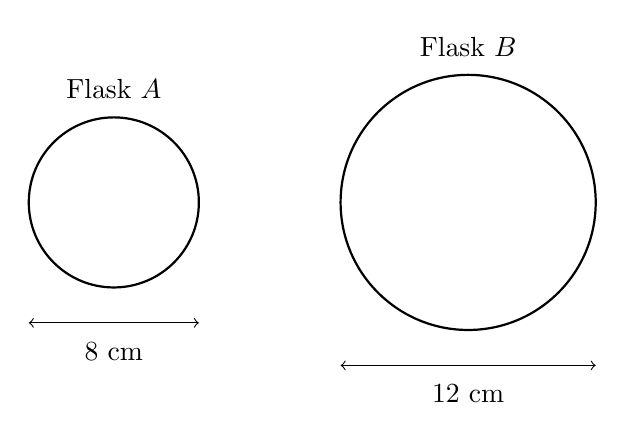
\begin{tikzpicture}[scale=0.9]
    % Flask A (smaller)
    \draw[thick] (0,0) circle (1.2cm);
    \draw[<->] (-1.2,-1.7) -- (1.2,-1.7);
    \node at (0,-2.1) {$8$ cm};
    \node at (0,1.6) {Flask $A$};

    % Flask B (larger)
    \draw[thick] (5,0) circle (1.8cm);
    \draw[<->] (3.2,-2.3) -- (6.8,-2.3);
    \node at (5,-2.7) {$12$ cm};
    \node at (5,2.2) {Flask $B$};
\end{tikzpicture}
\end{center}

\noindent The curved surface of flask $A$ has an area of $201$ cm$^2$.

\begin{enumerate}
    \item[(a)] Find the linear scale factor from flask $A$ to flask $B$.
    \vspace{2.5cm}
    \answerplain{1}

    \item[(b)] Work out the curved surface area of flask $B$.

    Give your answer to 3 significant figures.
    \vspace{5cm}
    \answerunit{$\text{cm}^2$}{3}
\end{enumerate}
\end{question}
